\documentclass[violet,handout]{beamer}
%\usepackage{xypic}
%\usepackage{czech,latin2}
%\usepackage[dvips]{graphicx}
%\usepackage{color}


%\usepackage[verbose,absolute,overlay]{textpos}
%\usepackage{pgf,pgfarrows,pgfnodes,pgfautomata,pgfheaps,pgfshade,hyperref}
%
\usepackage[utf8]{inputenc}
\usepackage{amsfonts}
\usepackage{graphicx}
%\usepackage[all]{xy}
%
\usetheme{Madrid}
\usepackage[english]{babel}
%
\font\eufm=eufm10  scaled 1300
\font\eusb=eusb10  scaled 1300
\font\eurb=eurb10  scaled 1300

%\newtheorem{dfn}{Definition}
%\newtheorem{thm}[dfn]{Theorem}
%\newtheorem{pro}[dfn]{Proposition}
%\newtheorem{cor}[dfn]{Corollary}
%\newtheorem{exm}{Example}
%\newtheorem{lem}[dfn]{Lemma}
\newtheorem{conjecture}{Conjecture}

\def\A{{\mathbb A}}
\def\B{{\mathbb B}}
\def\C{{\mathcal B}}
\def\algA{{\mathbf A}}
\def\algB{{\mathbf B}}
\def\Arrr{{\mathcal R}}
\def\Rplus{R^{+}}
\def\Rminus{R^{-}}
\def\M{{\mathcal M}}
\def\AND{\mathop{\wedge}}
\let\meet\wedge
\def\CSP{\operatorname{CSP}}
\def\Inv{\operatorname{Inv}}
\def\Pol{\operatorname{Pol}}
\def\Datalog{\operatorname{DATALOG}}
\def\sinks{\operatorname{sinks}}
\def\sources{\operatorname{sources}}
\def\var{\operatorname{var}}
\def\absorbs{\operatorname{\trianglelefteq}}
\def\Gabsorbs{\operatorname{\trianglelefteq_G}}
\def\Jabsorbs{\operatorname{\trianglelefteq_J}}
\def\zet{{\mathbb Z}}
\def\en{{\mathbb N}}

\setbeamercovered{transparent} % ???

\def\Prob{\operatorname{P}}

\title{How to decide absorption}
\author[AK \& LB]{Alexandr Kazda\\ (joint work with Libor Barto)}
\institute[Vanderbilt] {Department of Mathematics\\ Vanderbilt
University}
\date{October 5th 2013}
%
\begin{document}
%
\begin{frame}
   \titlepage
\end{frame}


\section{Introduction}
\begin{frame}
\frametitle{What is absorption?}
\pause
\begin{definition} [Libor Barto, Marcin Kozik]
  Let $\algB\leq \algA$ be algebras. We say that $\algB$ \alert{absorbs} $\algA$ if there exists a
  term $t$ in $\algA$ such that for any $b_1,\dots,b_n\in B, a\in A$ we have:
  \begin{align*}
    t(a,a,a,\dots,a)&=a\\
    t(a,b_2,b_3,\dots,b_{n-1},b_n)&\in B\\
    t(b_1,a,b_3,\dots,b_{n-1},b_n)&\in B\\
    \vdots\\
    t(b_1,b_2,b_3,\dots,b_{n-1},a)&\in B
  \end{align*}
\end{definition}
\end{frame}
\begin{frame}
  \frametitle{Ok, but what \emph{is} absorption?}
\begin{itemize}
  \pause\item If $0$ is the minimal element of a finite semilattice
    $(L,\meet)$, then
    $\{0\}$ absorbs $L$; absorption term is $t(x_1,x_2)=x_1\meet x_2$.
\pause\item If $\algA$ is an algebra with a majority term $m$, then every singleton is an
  absorbing subalgebra; absorption term is $m$.
\pause\item If $\algA$ is any algebra, then always $\algA\absorbs \algA$.
\pause\item If $\algA$ is an abelian group, then $\algA$ has no proper absorbing
  subalgebra.
\end{itemize}
\end{frame}
\begin{frame}
  \frametitle{Deciding absorption}
  \begin{itemize}
    \pause\item Let $\algA$ be an idempotent finite algebra. Then $\algA$ has an NU term iff
      every singleton $\{a\}$ absorbs $\algA$.
     \pause\item Miklós Maróti, Libor Barto, Dmitriy Zhuk: We can decide whether a finite 
       algebra $\algA$ has an NU term.
    \pause\item Problem: Given $\algB\leq \algA$, can we decide if $\algB\absorbs \algA$?
    \pause\item Libor Barto, Jakub Bulín: Yes, if $\algA$ is finitely related.
    \pause\item What about if $\algA$ is given by a finitely many
      operations instead?
  \end{itemize}
    \end{frame}

    \begin{frame}
      \frametitle{Blockers}
      \begin{itemize}
	\pause\item Let $\algB\absorbs \algA$ with absorption term $t$.
	\pause\item We call $(C,D)$ a \alert{blocker} for $\algB$ if
	  \begin{itemize}
	    \item $\emptyset\neq D\subset C$,
	    \item $C\cap B\neq \emptyset$,
	    \item $D\cap B=\emptyset$,
	    \item $\{(x_1,\dots,x_n)\in C^n :\exists i,\,
	  x_i\in D\} \leq A^n$ for every $n\in\en$.
      \end{itemize}
	\pause\item If $\algB\absorbs \algA$, then there is no blocker for $\algB$.
      \end{itemize}
    \end{frame}
%25 min
    \begin{frame}
      \frametitle{No blockers $\Rightarrow$ absorption?}
      \begin{itemize}
	\pause\item Given idempotent $\algA$ with finitely many operations, we can test if there are
	  no blockers for $\algB$.
	\pause\item However, we can have no blockers and no absorption: Consider
	  $\algA=(\zet_2,m)$, where $m(x,y,z)=x+y+z \pmod 2$.
      \end{itemize}
    \end{frame}
%35 min
    \begin{frame}
      \frametitle{Jónsson absorption}
  \begin{itemize}
      \pause\item Weaker notion of absorption inspired by terms for congruence
	distributivity.
    \pause\item Let $\algB\leq \algA$.  Then $\algB\absorbs_J \algA$ if there exist idempotent 
      terms $d_0,d_1,\dots,d_n$ such that:
 \begin{align*}
     \forall i=0,\dots,n,\,d_i(B,A,B)&\subset B\\
     d_0(x,y,z)&=x\\
     d_i(x,y,y)&=d_{i+1}(x,y,y)\; \text{for $i$ even}\\
     d_i(x,x,y)&=d_{i+1}(x,x,y)\; \text{for $i$ odd}\\
     d_n(x,y,z)&=z.
 \end{align*}
 \end{itemize}
    \end{frame}

    \begin{frame}
      \frametitle{Putting it all together}
      \center{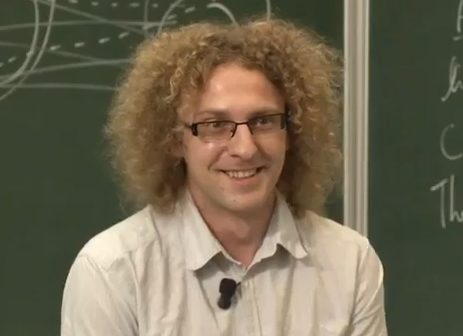
\includegraphics[width=1.5in]{2012barto.jpg}}
      \pause
      \begin{theorem}
	Let $\algA$ be a finite idempotent algebra, $\algB\leq \algA$.
	Then $\algB\absorbs \algA$ iff there is no blocker for $\algB$ and $\algB\absorbs_J \algA$.
      \end{theorem}\pause
      \begin{corollary}
      We can decide $\algB\absorbs \algA$ algorithmically for idempotent algebras.
    \end{corollary}
    \end{frame}
%55 min
    \begin{frame}
      \begin{itemize}
	  \frametitle{Nonidempotent algebras}
	\pause\item If $\algA$ is not idempotent, we would also like to decide
	  to absorption.
	  \pause\item Problem with taking the idempotent reduct: We might lose 
	    the generators of the clone of $\algA$.
	  \pause\item Imitating some of Dmitriy Zhuk's ideas should give us an
	    algorithm anyway\dots
      \end{itemize}
    \end{frame}
\begin{frame}
\centerline{Thank you for your attention.}
\end{frame}
\end{document}

